% Created by tikzDevice version 0.8.1 on 2015-08-26 15:58:59
% !TEX encoding = UTF-8 Unicode
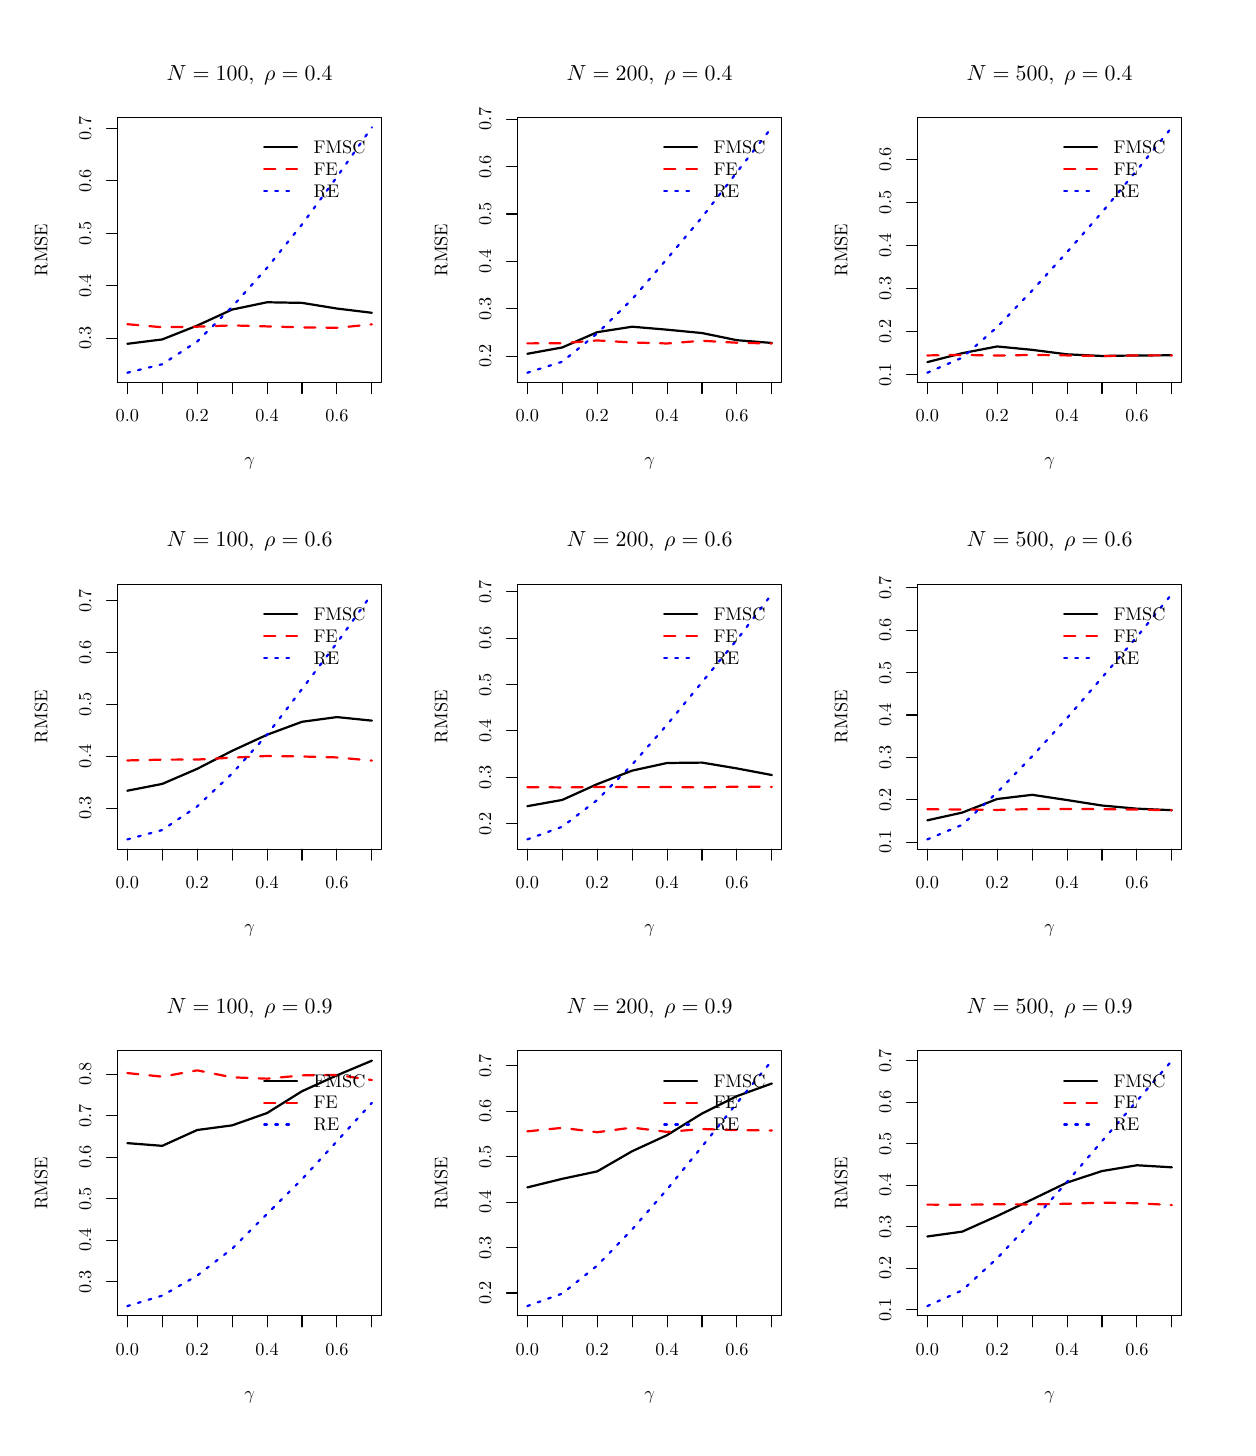
\begin{tikzpicture}[x=1pt,y=1pt]
\definecolor{fillColor}{RGB}{255,255,255}
\path[use as bounding box,fill=fillColor,fill opacity=0.00] (0,0) rectangle (433.62,505.89);
\begin{scope}
\path[clip] ( 32.47,377.65) rectangle (127.91,473.42);
\definecolor{drawColor}{RGB}{0,0,0}

\path[draw=drawColor,line width= 0.8pt,line join=round,line cap=round] ( 36.01,391.65) --
	( 48.63,393.23) --
	( 61.25,398.23) --
	( 73.88,404.03) --
	( 86.50,406.66) --
	( 99.13,406.44) --
	(111.75,404.39) --
	(124.37,402.86);
\end{scope}
\begin{scope}
\path[clip] (  0.00,  0.00) rectangle (433.62,505.89);
\definecolor{drawColor}{RGB}{0,0,0}

\path[draw=drawColor,line width= 0.4pt,line join=round,line cap=round] ( 36.01,377.65) -- (124.37,377.65);

\path[draw=drawColor,line width= 0.4pt,line join=round,line cap=round] ( 36.01,377.65) -- ( 36.01,373.69);

\path[draw=drawColor,line width= 0.4pt,line join=round,line cap=round] ( 48.63,377.65) -- ( 48.63,373.69);

\path[draw=drawColor,line width= 0.4pt,line join=round,line cap=round] ( 61.25,377.65) -- ( 61.25,373.69);

\path[draw=drawColor,line width= 0.4pt,line join=round,line cap=round] ( 73.88,377.65) -- ( 73.88,373.69);

\path[draw=drawColor,line width= 0.4pt,line join=round,line cap=round] ( 86.50,377.65) -- ( 86.50,373.69);

\path[draw=drawColor,line width= 0.4pt,line join=round,line cap=round] ( 99.13,377.65) -- ( 99.13,373.69);

\path[draw=drawColor,line width= 0.4pt,line join=round,line cap=round] (111.75,377.65) -- (111.75,373.69);

\path[draw=drawColor,line width= 0.4pt,line join=round,line cap=round] (124.37,377.65) -- (124.37,373.69);

\node[text=drawColor,anchor=base,inner sep=0pt, outer sep=0pt, scale=  0.66] at ( 36.01,363.40) {0.0};

\node[text=drawColor,anchor=base,inner sep=0pt, outer sep=0pt, scale=  0.66] at ( 61.25,363.40) {0.2};

\node[text=drawColor,anchor=base,inner sep=0pt, outer sep=0pt, scale=  0.66] at ( 86.50,363.40) {0.4};

\node[text=drawColor,anchor=base,inner sep=0pt, outer sep=0pt, scale=  0.66] at (111.75,363.40) {0.6};

\path[draw=drawColor,line width= 0.4pt,line join=round,line cap=round] ( 32.47,393.65) -- ( 32.47,469.46);

\path[draw=drawColor,line width= 0.4pt,line join=round,line cap=round] ( 32.47,393.65) -- ( 28.51,393.65);

\path[draw=drawColor,line width= 0.4pt,line join=round,line cap=round] ( 32.47,412.61) -- ( 28.51,412.61);

\path[draw=drawColor,line width= 0.4pt,line join=round,line cap=round] ( 32.47,431.56) -- ( 28.51,431.56);

\path[draw=drawColor,line width= 0.4pt,line join=round,line cap=round] ( 32.47,450.51) -- ( 28.51,450.51);

\path[draw=drawColor,line width= 0.4pt,line join=round,line cap=round] ( 32.47,469.46) -- ( 28.51,469.46);

\node[text=drawColor,rotate= 90.00,anchor=base,inner sep=0pt, outer sep=0pt, scale=  0.66] at ( 22.97,393.65) {0.3};

\node[text=drawColor,rotate= 90.00,anchor=base,inner sep=0pt, outer sep=0pt, scale=  0.66] at ( 22.97,412.61) {0.4};

\node[text=drawColor,rotate= 90.00,anchor=base,inner sep=0pt, outer sep=0pt, scale=  0.66] at ( 22.97,431.56) {0.5};

\node[text=drawColor,rotate= 90.00,anchor=base,inner sep=0pt, outer sep=0pt, scale=  0.66] at ( 22.97,450.51) {0.6};

\node[text=drawColor,rotate= 90.00,anchor=base,inner sep=0pt, outer sep=0pt, scale=  0.66] at ( 22.97,469.46) {0.7};

\path[draw=drawColor,line width= 0.4pt,line join=round,line cap=round] ( 32.47,377.65) --
	(127.91,377.65) --
	(127.91,473.42) --
	( 32.47,473.42) --
	( 32.47,377.65);
\end{scope}
\begin{scope}
\path[clip] (  0.00,337.26) rectangle (144.54,505.89);
\definecolor{drawColor}{RGB}{0,0,0}

\node[text=drawColor,anchor=base,inner sep=0pt, outer sep=0pt, scale=  0.79] at ( 80.19,486.92) {\bfseries $N=100, \;\rho=0.4$};

\node[text=drawColor,anchor=base,inner sep=0pt, outer sep=0pt, scale=  0.66] at ( 80.19,347.56) {$\gamma$};

\node[text=drawColor,rotate= 90.00,anchor=base,inner sep=0pt, outer sep=0pt, scale=  0.66] at (  7.13,425.53) {RMSE};
\end{scope}
\begin{scope}
\path[clip] ( 32.47,377.65) rectangle (127.91,473.42);
\definecolor{drawColor}{RGB}{255,0,0}

\path[draw=drawColor,line width= 0.8pt,dash pattern=on 4pt off 4pt ,line join=round,line cap=round] ( 36.01,398.73) --
	( 48.63,397.63) --
	( 61.25,397.84) --
	( 73.88,398.30) --
	( 86.50,397.94) --
	( 99.13,397.59) --
	(111.75,397.41) --
	(124.37,398.69);
\definecolor{drawColor}{RGB}{0,0,255}

\path[draw=drawColor,line width= 0.8pt,dash pattern=on 1pt off 3pt ,line join=round,line cap=round] ( 36.01,381.20) --
	( 48.63,384.27) --
	( 61.25,392.48) --
	( 73.88,405.01) --
	( 86.50,419.12) --
	( 99.13,434.78) --
	(111.75,451.95) --
	(124.37,469.87);
\definecolor{drawColor}{RGB}{0,0,0}

\path[draw=drawColor,line width= 0.8pt,line join=round,line cap=round] ( 85.47,462.63) -- ( 97.35,462.63);
\definecolor{drawColor}{RGB}{255,0,0}

\path[draw=drawColor,line width= 0.8pt,dash pattern=on 4pt off 4pt ,line join=round,line cap=round] ( 85.47,454.71) -- ( 97.35,454.71);
\definecolor{drawColor}{RGB}{0,0,255}

\path[draw=drawColor,line width= 0.8pt,dash pattern=on 1pt off 3pt ,line join=round,line cap=round] ( 85.47,446.79) -- ( 97.35,446.79);
\definecolor{drawColor}{RGB}{0,0,0}

\node[text=drawColor,anchor=base west,inner sep=0pt, outer sep=0pt, scale=  0.66] at (103.29,460.35) {FMSC};

\node[text=drawColor,anchor=base west,inner sep=0pt, outer sep=0pt, scale=  0.66] at (103.29,452.43) {FE};

\node[text=drawColor,anchor=base west,inner sep=0pt, outer sep=0pt, scale=  0.66] at (103.29,444.51) {RE};
\end{scope}
\begin{scope}
\path[clip] (177.01,377.65) rectangle (272.45,473.42);
\definecolor{drawColor}{RGB}{0,0,0}

\path[draw=drawColor,line width= 0.8pt,line join=round,line cap=round] (180.55,388.04) --
	(193.17,390.33) --
	(205.79,395.85) --
	(218.42,397.83) --
	(231.04,396.75) --
	(243.67,395.54) --
	(256.29,392.95) --
	(268.91,391.96);
\end{scope}
\begin{scope}
\path[clip] (  0.00,  0.00) rectangle (433.62,505.89);
\definecolor{drawColor}{RGB}{0,0,0}

\path[draw=drawColor,line width= 0.4pt,line join=round,line cap=round] (180.55,377.65) -- (268.91,377.65);

\path[draw=drawColor,line width= 0.4pt,line join=round,line cap=round] (180.55,377.65) -- (180.55,373.69);

\path[draw=drawColor,line width= 0.4pt,line join=round,line cap=round] (193.17,377.65) -- (193.17,373.69);

\path[draw=drawColor,line width= 0.4pt,line join=round,line cap=round] (205.79,377.65) -- (205.79,373.69);

\path[draw=drawColor,line width= 0.4pt,line join=round,line cap=round] (218.42,377.65) -- (218.42,373.69);

\path[draw=drawColor,line width= 0.4pt,line join=round,line cap=round] (231.04,377.65) -- (231.04,373.69);

\path[draw=drawColor,line width= 0.4pt,line join=round,line cap=round] (243.67,377.65) -- (243.67,373.69);

\path[draw=drawColor,line width= 0.4pt,line join=round,line cap=round] (256.29,377.65) -- (256.29,373.69);

\path[draw=drawColor,line width= 0.4pt,line join=round,line cap=round] (268.91,377.65) -- (268.91,373.69);

\node[text=drawColor,anchor=base,inner sep=0pt, outer sep=0pt, scale=  0.66] at (180.55,363.40) {0.0};

\node[text=drawColor,anchor=base,inner sep=0pt, outer sep=0pt, scale=  0.66] at (205.79,363.40) {0.2};

\node[text=drawColor,anchor=base,inner sep=0pt, outer sep=0pt, scale=  0.66] at (231.04,363.40) {0.4};

\node[text=drawColor,anchor=base,inner sep=0pt, outer sep=0pt, scale=  0.66] at (256.29,363.40) {0.6};

\path[draw=drawColor,line width= 0.4pt,line join=round,line cap=round] (177.01,387.19) -- (177.01,472.82);

\path[draw=drawColor,line width= 0.4pt,line join=round,line cap=round] (177.01,387.19) -- (173.05,387.19);

\path[draw=drawColor,line width= 0.4pt,line join=round,line cap=round] (177.01,404.31) -- (173.05,404.31);

\path[draw=drawColor,line width= 0.4pt,line join=round,line cap=round] (177.01,421.44) -- (173.05,421.44);

\path[draw=drawColor,line width= 0.4pt,line join=round,line cap=round] (177.01,438.57) -- (173.05,438.57);

\path[draw=drawColor,line width= 0.4pt,line join=round,line cap=round] (177.01,455.69) -- (173.05,455.69);

\path[draw=drawColor,line width= 0.4pt,line join=round,line cap=round] (177.01,472.82) -- (173.05,472.82);

\node[text=drawColor,rotate= 90.00,anchor=base,inner sep=0pt, outer sep=0pt, scale=  0.66] at (167.51,387.19) {0.2};

\node[text=drawColor,rotate= 90.00,anchor=base,inner sep=0pt, outer sep=0pt, scale=  0.66] at (167.51,404.31) {0.3};

\node[text=drawColor,rotate= 90.00,anchor=base,inner sep=0pt, outer sep=0pt, scale=  0.66] at (167.51,421.44) {0.4};

\node[text=drawColor,rotate= 90.00,anchor=base,inner sep=0pt, outer sep=0pt, scale=  0.66] at (167.51,438.57) {0.5};

\node[text=drawColor,rotate= 90.00,anchor=base,inner sep=0pt, outer sep=0pt, scale=  0.66] at (167.51,455.69) {0.6};

\node[text=drawColor,rotate= 90.00,anchor=base,inner sep=0pt, outer sep=0pt, scale=  0.66] at (167.51,472.82) {0.7};

\path[draw=drawColor,line width= 0.4pt,line join=round,line cap=round] (177.01,377.65) --
	(272.45,377.65) --
	(272.45,473.42) --
	(177.01,473.42) --
	(177.01,377.65);
\end{scope}
\begin{scope}
\path[clip] (144.54,337.26) rectangle (289.08,505.89);
\definecolor{drawColor}{RGB}{0,0,0}

\node[text=drawColor,anchor=base,inner sep=0pt, outer sep=0pt, scale=  0.79] at (224.73,486.92) {\bfseries $N=200, \;\rho=0.4$};

\node[text=drawColor,anchor=base,inner sep=0pt, outer sep=0pt, scale=  0.66] at (224.73,347.56) {$\gamma$};

\node[text=drawColor,rotate= 90.00,anchor=base,inner sep=0pt, outer sep=0pt, scale=  0.66] at (151.67,425.53) {RMSE};
\end{scope}
\begin{scope}
\path[clip] (177.01,377.65) rectangle (272.45,473.42);
\definecolor{drawColor}{RGB}{255,0,0}

\path[draw=drawColor,line width= 0.8pt,dash pattern=on 4pt off 4pt ,line join=round,line cap=round] (180.55,391.80) --
	(193.17,391.87) --
	(205.79,392.87) --
	(218.42,392.13) --
	(231.04,391.77) --
	(243.67,392.75) --
	(256.29,392.04) --
	(268.91,391.76);
\definecolor{drawColor}{RGB}{0,0,255}

\path[draw=drawColor,line width= 0.8pt,dash pattern=on 1pt off 3pt ,line join=round,line cap=round] (180.55,381.20) --
	(193.17,385.18) --
	(205.79,395.40) --
	(218.42,407.76) --
	(231.04,422.36) --
	(243.67,437.38) --
	(256.29,453.69) --
	(268.91,469.87);
\definecolor{drawColor}{RGB}{0,0,0}

\path[draw=drawColor,line width= 0.8pt,line join=round,line cap=round] (230.01,462.63) -- (241.89,462.63);
\definecolor{drawColor}{RGB}{255,0,0}

\path[draw=drawColor,line width= 0.8pt,dash pattern=on 4pt off 4pt ,line join=round,line cap=round] (230.01,454.71) -- (241.89,454.71);
\definecolor{drawColor}{RGB}{0,0,255}

\path[draw=drawColor,line width= 0.8pt,dash pattern=on 1pt off 3pt ,line join=round,line cap=round] (230.01,446.79) -- (241.89,446.79);
\definecolor{drawColor}{RGB}{0,0,0}

\node[text=drawColor,anchor=base west,inner sep=0pt, outer sep=0pt, scale=  0.66] at (247.83,460.35) {FMSC};

\node[text=drawColor,anchor=base west,inner sep=0pt, outer sep=0pt, scale=  0.66] at (247.83,452.43) {FE};

\node[text=drawColor,anchor=base west,inner sep=0pt, outer sep=0pt, scale=  0.66] at (247.83,444.51) {RE};
\end{scope}
\begin{scope}
\path[clip] (321.55,377.65) rectangle (416.99,473.42);
\definecolor{drawColor}{RGB}{0,0,0}

\path[draw=drawColor,line width= 0.8pt,line join=round,line cap=round] (325.09,385.03) --
	(337.71,388.26) --
	(350.33,390.69) --
	(362.96,389.47) --
	(375.58,387.85) --
	(388.21,387.26) --
	(400.83,387.44) --
	(413.45,387.49);
\end{scope}
\begin{scope}
\path[clip] (  0.00,  0.00) rectangle (433.62,505.89);
\definecolor{drawColor}{RGB}{0,0,0}

\path[draw=drawColor,line width= 0.4pt,line join=round,line cap=round] (325.09,377.65) -- (413.45,377.65);

\path[draw=drawColor,line width= 0.4pt,line join=round,line cap=round] (325.09,377.65) -- (325.09,373.69);

\path[draw=drawColor,line width= 0.4pt,line join=round,line cap=round] (337.71,377.65) -- (337.71,373.69);

\path[draw=drawColor,line width= 0.4pt,line join=round,line cap=round] (350.33,377.65) -- (350.33,373.69);

\path[draw=drawColor,line width= 0.4pt,line join=round,line cap=round] (362.96,377.65) -- (362.96,373.69);

\path[draw=drawColor,line width= 0.4pt,line join=round,line cap=round] (375.58,377.65) -- (375.58,373.69);

\path[draw=drawColor,line width= 0.4pt,line join=round,line cap=round] (388.21,377.65) -- (388.21,373.69);

\path[draw=drawColor,line width= 0.4pt,line join=round,line cap=round] (400.83,377.65) -- (400.83,373.69);

\path[draw=drawColor,line width= 0.4pt,line join=round,line cap=round] (413.45,377.65) -- (413.45,373.69);

\node[text=drawColor,anchor=base,inner sep=0pt, outer sep=0pt, scale=  0.66] at (325.09,363.40) {0.0};

\node[text=drawColor,anchor=base,inner sep=0pt, outer sep=0pt, scale=  0.66] at (350.33,363.40) {0.2};

\node[text=drawColor,anchor=base,inner sep=0pt, outer sep=0pt, scale=  0.66] at (375.58,363.40) {0.4};

\node[text=drawColor,anchor=base,inner sep=0pt, outer sep=0pt, scale=  0.66] at (400.83,363.40) {0.6};

\path[draw=drawColor,line width= 0.4pt,line join=round,line cap=round] (321.55,380.55) -- (321.55,458.29);

\path[draw=drawColor,line width= 0.4pt,line join=round,line cap=round] (321.55,380.55) -- (317.59,380.55);

\path[draw=drawColor,line width= 0.4pt,line join=round,line cap=round] (321.55,396.10) -- (317.59,396.10);

\path[draw=drawColor,line width= 0.4pt,line join=round,line cap=round] (321.55,411.65) -- (317.59,411.65);

\path[draw=drawColor,line width= 0.4pt,line join=round,line cap=round] (321.55,427.19) -- (317.59,427.19);

\path[draw=drawColor,line width= 0.4pt,line join=round,line cap=round] (321.55,442.74) -- (317.59,442.74);

\path[draw=drawColor,line width= 0.4pt,line join=round,line cap=round] (321.55,458.29) -- (317.59,458.29);

\node[text=drawColor,rotate= 90.00,anchor=base,inner sep=0pt, outer sep=0pt, scale=  0.66] at (312.05,380.55) {0.1};

\node[text=drawColor,rotate= 90.00,anchor=base,inner sep=0pt, outer sep=0pt, scale=  0.66] at (312.05,396.10) {0.2};

\node[text=drawColor,rotate= 90.00,anchor=base,inner sep=0pt, outer sep=0pt, scale=  0.66] at (312.05,411.65) {0.3};

\node[text=drawColor,rotate= 90.00,anchor=base,inner sep=0pt, outer sep=0pt, scale=  0.66] at (312.05,427.19) {0.4};

\node[text=drawColor,rotate= 90.00,anchor=base,inner sep=0pt, outer sep=0pt, scale=  0.66] at (312.05,442.74) {0.5};

\node[text=drawColor,rotate= 90.00,anchor=base,inner sep=0pt, outer sep=0pt, scale=  0.66] at (312.05,458.29) {0.6};

\path[draw=drawColor,line width= 0.4pt,line join=round,line cap=round] (321.55,377.65) --
	(416.99,377.65) --
	(416.99,473.42) --
	(321.55,473.42) --
	(321.55,377.65);
\end{scope}
\begin{scope}
\path[clip] (289.08,337.26) rectangle (433.62,505.89);
\definecolor{drawColor}{RGB}{0,0,0}

\node[text=drawColor,anchor=base,inner sep=0pt, outer sep=0pt, scale=  0.79] at (369.27,486.92) {\bfseries $N=500, \;\rho=0.4$};

\node[text=drawColor,anchor=base,inner sep=0pt, outer sep=0pt, scale=  0.66] at (369.27,347.56) {$\gamma$};

\node[text=drawColor,rotate= 90.00,anchor=base,inner sep=0pt, outer sep=0pt, scale=  0.66] at (296.21,425.53) {RMSE};
\end{scope}
\begin{scope}
\path[clip] (321.55,377.65) rectangle (416.99,473.42);
\definecolor{drawColor}{RGB}{255,0,0}

\path[draw=drawColor,line width= 0.8pt,dash pattern=on 4pt off 4pt ,line join=round,line cap=round] (325.09,387.45) --
	(337.71,387.64) --
	(350.33,387.40) --
	(362.96,387.63) --
	(375.58,387.46) --
	(388.21,387.22) --
	(400.83,387.44) --
	(413.45,387.49);
\definecolor{drawColor}{RGB}{0,0,255}

\path[draw=drawColor,line width= 0.8pt,dash pattern=on 1pt off 3pt ,line join=round,line cap=round] (325.09,381.20) --
	(337.71,386.65) --
	(350.33,397.71) --
	(362.96,410.89) --
	(375.58,424.79) --
	(388.21,439.18) --
	(400.83,454.41) --
	(413.45,469.87);
\definecolor{drawColor}{RGB}{0,0,0}

\path[draw=drawColor,line width= 0.8pt,line join=round,line cap=round] (374.55,462.63) -- (386.43,462.63);
\definecolor{drawColor}{RGB}{255,0,0}

\path[draw=drawColor,line width= 0.8pt,dash pattern=on 4pt off 4pt ,line join=round,line cap=round] (374.55,454.71) -- (386.43,454.71);
\definecolor{drawColor}{RGB}{0,0,255}

\path[draw=drawColor,line width= 0.8pt,dash pattern=on 1pt off 3pt ,line join=round,line cap=round] (374.55,446.79) -- (386.43,446.79);
\definecolor{drawColor}{RGB}{0,0,0}

\node[text=drawColor,anchor=base west,inner sep=0pt, outer sep=0pt, scale=  0.66] at (392.37,460.35) {FMSC};

\node[text=drawColor,anchor=base west,inner sep=0pt, outer sep=0pt, scale=  0.66] at (392.37,452.43) {FE};

\node[text=drawColor,anchor=base west,inner sep=0pt, outer sep=0pt, scale=  0.66] at (392.37,444.51) {RE};
\end{scope}
\begin{scope}
\path[clip] ( 32.47,209.02) rectangle (127.91,304.79);
\definecolor{drawColor}{RGB}{0,0,0}

\path[draw=drawColor,line width= 0.8pt,line join=round,line cap=round] ( 36.01,230.16) --
	( 48.63,232.62) --
	( 61.25,238.07) --
	( 73.88,244.57) --
	( 86.50,250.38) --
	( 99.13,255.07) --
	(111.75,256.77) --
	(124.37,255.48);
\end{scope}
\begin{scope}
\path[clip] (  0.00,  0.00) rectangle (433.62,505.89);
\definecolor{drawColor}{RGB}{0,0,0}

\path[draw=drawColor,line width= 0.4pt,line join=round,line cap=round] ( 36.01,209.02) -- (124.37,209.02);

\path[draw=drawColor,line width= 0.4pt,line join=round,line cap=round] ( 36.01,209.02) -- ( 36.01,205.06);

\path[draw=drawColor,line width= 0.4pt,line join=round,line cap=round] ( 48.63,209.02) -- ( 48.63,205.06);

\path[draw=drawColor,line width= 0.4pt,line join=round,line cap=round] ( 61.25,209.02) -- ( 61.25,205.06);

\path[draw=drawColor,line width= 0.4pt,line join=round,line cap=round] ( 73.88,209.02) -- ( 73.88,205.06);

\path[draw=drawColor,line width= 0.4pt,line join=round,line cap=round] ( 86.50,209.02) -- ( 86.50,205.06);

\path[draw=drawColor,line width= 0.4pt,line join=round,line cap=round] ( 99.13,209.02) -- ( 99.13,205.06);

\path[draw=drawColor,line width= 0.4pt,line join=round,line cap=round] (111.75,209.02) -- (111.75,205.06);

\path[draw=drawColor,line width= 0.4pt,line join=round,line cap=round] (124.37,209.02) -- (124.37,205.06);

\node[text=drawColor,anchor=base,inner sep=0pt, outer sep=0pt, scale=  0.66] at ( 36.01,194.77) {0.0};

\node[text=drawColor,anchor=base,inner sep=0pt, outer sep=0pt, scale=  0.66] at ( 61.25,194.77) {0.2};

\node[text=drawColor,anchor=base,inner sep=0pt, outer sep=0pt, scale=  0.66] at ( 86.50,194.77) {0.4};

\node[text=drawColor,anchor=base,inner sep=0pt, outer sep=0pt, scale=  0.66] at (111.75,194.77) {0.6};

\path[draw=drawColor,line width= 0.4pt,line join=round,line cap=round] ( 32.47,223.81) -- ( 32.47,298.88);

\path[draw=drawColor,line width= 0.4pt,line join=round,line cap=round] ( 32.47,223.81) -- ( 28.51,223.81);

\path[draw=drawColor,line width= 0.4pt,line join=round,line cap=round] ( 32.47,242.58) -- ( 28.51,242.58);

\path[draw=drawColor,line width= 0.4pt,line join=round,line cap=round] ( 32.47,261.35) -- ( 28.51,261.35);

\path[draw=drawColor,line width= 0.4pt,line join=round,line cap=round] ( 32.47,280.12) -- ( 28.51,280.12);

\path[draw=drawColor,line width= 0.4pt,line join=round,line cap=round] ( 32.47,298.88) -- ( 28.51,298.88);

\node[text=drawColor,rotate= 90.00,anchor=base,inner sep=0pt, outer sep=0pt, scale=  0.66] at ( 22.97,223.81) {0.3};

\node[text=drawColor,rotate= 90.00,anchor=base,inner sep=0pt, outer sep=0pt, scale=  0.66] at ( 22.97,242.58) {0.4};

\node[text=drawColor,rotate= 90.00,anchor=base,inner sep=0pt, outer sep=0pt, scale=  0.66] at ( 22.97,261.35) {0.5};

\node[text=drawColor,rotate= 90.00,anchor=base,inner sep=0pt, outer sep=0pt, scale=  0.66] at ( 22.97,280.12) {0.6};

\node[text=drawColor,rotate= 90.00,anchor=base,inner sep=0pt, outer sep=0pt, scale=  0.66] at ( 22.97,298.88) {0.7};

\path[draw=drawColor,line width= 0.4pt,line join=round,line cap=round] ( 32.47,209.02) --
	(127.91,209.02) --
	(127.91,304.79) --
	( 32.47,304.79) --
	( 32.47,209.02);
\end{scope}
\begin{scope}
\path[clip] (  0.00,168.63) rectangle (144.54,337.26);
\definecolor{drawColor}{RGB}{0,0,0}

\node[text=drawColor,anchor=base,inner sep=0pt, outer sep=0pt, scale=  0.79] at ( 80.19,318.29) {\bfseries $N=100, \;\rho=0.6$};

\node[text=drawColor,anchor=base,inner sep=0pt, outer sep=0pt, scale=  0.66] at ( 80.19,178.93) {$\gamma$};

\node[text=drawColor,rotate= 90.00,anchor=base,inner sep=0pt, outer sep=0pt, scale=  0.66] at (  7.13,256.90) {RMSE};
\end{scope}
\begin{scope}
\path[clip] ( 32.47,209.02) rectangle (127.91,304.79);
\definecolor{drawColor}{RGB}{255,0,0}

\path[draw=drawColor,line width= 0.8pt,dash pattern=on 4pt off 4pt ,line join=round,line cap=round] ( 36.01,241.10) --
	( 48.63,241.39) --
	( 61.25,241.42) --
	( 73.88,242.10) --
	( 86.50,242.71) --
	( 99.13,242.53) --
	(111.75,242.19) --
	(124.37,241.04);
\definecolor{drawColor}{RGB}{0,0,255}

\path[draw=drawColor,line width= 0.8pt,dash pattern=on 1pt off 3pt ,line join=round,line cap=round] ( 36.01,212.57) --
	( 48.63,215.95) --
	( 61.25,224.49) --
	( 73.88,236.37) --
	( 86.50,250.38) --
	( 99.13,266.91) --
	(111.75,283.57) --
	(124.37,301.24);
\definecolor{drawColor}{RGB}{0,0,0}

\path[draw=drawColor,line width= 0.8pt,line join=round,line cap=round] ( 85.47,294.00) -- ( 97.35,294.00);
\definecolor{drawColor}{RGB}{255,0,0}

\path[draw=drawColor,line width= 0.8pt,dash pattern=on 4pt off 4pt ,line join=round,line cap=round] ( 85.47,286.08) -- ( 97.35,286.08);
\definecolor{drawColor}{RGB}{0,0,255}

\path[draw=drawColor,line width= 0.8pt,dash pattern=on 1pt off 3pt ,line join=round,line cap=round] ( 85.47,278.16) -- ( 97.35,278.16);
\definecolor{drawColor}{RGB}{0,0,0}

\node[text=drawColor,anchor=base west,inner sep=0pt, outer sep=0pt, scale=  0.66] at (103.29,291.72) {FMSC};

\node[text=drawColor,anchor=base west,inner sep=0pt, outer sep=0pt, scale=  0.66] at (103.29,283.80) {FE};

\node[text=drawColor,anchor=base west,inner sep=0pt, outer sep=0pt, scale=  0.66] at (103.29,275.88) {RE};
\end{scope}
\begin{scope}
\path[clip] (177.01,209.02) rectangle (272.45,304.79);
\definecolor{drawColor}{RGB}{0,0,0}

\path[draw=drawColor,line width= 0.8pt,line join=round,line cap=round] (180.55,224.57) --
	(193.17,226.83) --
	(205.79,232.54) --
	(218.42,237.42) --
	(231.04,240.18) --
	(243.67,240.32) --
	(256.29,238.21) --
	(268.91,235.83);
\end{scope}
\begin{scope}
\path[clip] (  0.00,  0.00) rectangle (433.62,505.89);
\definecolor{drawColor}{RGB}{0,0,0}

\path[draw=drawColor,line width= 0.4pt,line join=round,line cap=round] (180.55,209.02) -- (268.91,209.02);

\path[draw=drawColor,line width= 0.4pt,line join=round,line cap=round] (180.55,209.02) -- (180.55,205.06);

\path[draw=drawColor,line width= 0.4pt,line join=round,line cap=round] (193.17,209.02) -- (193.17,205.06);

\path[draw=drawColor,line width= 0.4pt,line join=round,line cap=round] (205.79,209.02) -- (205.79,205.06);

\path[draw=drawColor,line width= 0.4pt,line join=round,line cap=round] (218.42,209.02) -- (218.42,205.06);

\path[draw=drawColor,line width= 0.4pt,line join=round,line cap=round] (231.04,209.02) -- (231.04,205.06);

\path[draw=drawColor,line width= 0.4pt,line join=round,line cap=round] (243.67,209.02) -- (243.67,205.06);

\path[draw=drawColor,line width= 0.4pt,line join=round,line cap=round] (256.29,209.02) -- (256.29,205.06);

\path[draw=drawColor,line width= 0.4pt,line join=round,line cap=round] (268.91,209.02) -- (268.91,205.06);

\node[text=drawColor,anchor=base,inner sep=0pt, outer sep=0pt, scale=  0.66] at (180.55,194.77) {0.0};

\node[text=drawColor,anchor=base,inner sep=0pt, outer sep=0pt, scale=  0.66] at (205.79,194.77) {0.2};

\node[text=drawColor,anchor=base,inner sep=0pt, outer sep=0pt, scale=  0.66] at (231.04,194.77) {0.4};

\node[text=drawColor,anchor=base,inner sep=0pt, outer sep=0pt, scale=  0.66] at (256.29,194.77) {0.6};

\path[draw=drawColor,line width= 0.4pt,line join=round,line cap=round] (177.01,218.24) -- (177.01,302.03);

\path[draw=drawColor,line width= 0.4pt,line join=round,line cap=round] (177.01,218.24) -- (173.05,218.24);

\path[draw=drawColor,line width= 0.4pt,line join=round,line cap=round] (177.01,235.00) -- (173.05,235.00);

\path[draw=drawColor,line width= 0.4pt,line join=round,line cap=round] (177.01,251.76) -- (173.05,251.76);

\path[draw=drawColor,line width= 0.4pt,line join=round,line cap=round] (177.01,268.52) -- (173.05,268.52);

\path[draw=drawColor,line width= 0.4pt,line join=round,line cap=round] (177.01,285.27) -- (173.05,285.27);

\path[draw=drawColor,line width= 0.4pt,line join=round,line cap=round] (177.01,302.03) -- (173.05,302.03);

\node[text=drawColor,rotate= 90.00,anchor=base,inner sep=0pt, outer sep=0pt, scale=  0.66] at (167.51,218.24) {0.2};

\node[text=drawColor,rotate= 90.00,anchor=base,inner sep=0pt, outer sep=0pt, scale=  0.66] at (167.51,235.00) {0.3};

\node[text=drawColor,rotate= 90.00,anchor=base,inner sep=0pt, outer sep=0pt, scale=  0.66] at (167.51,251.76) {0.4};

\node[text=drawColor,rotate= 90.00,anchor=base,inner sep=0pt, outer sep=0pt, scale=  0.66] at (167.51,268.52) {0.5};

\node[text=drawColor,rotate= 90.00,anchor=base,inner sep=0pt, outer sep=0pt, scale=  0.66] at (167.51,285.27) {0.6};

\node[text=drawColor,rotate= 90.00,anchor=base,inner sep=0pt, outer sep=0pt, scale=  0.66] at (167.51,302.03) {0.7};

\path[draw=drawColor,line width= 0.4pt,line join=round,line cap=round] (177.01,209.02) --
	(272.45,209.02) --
	(272.45,304.79) --
	(177.01,304.79) --
	(177.01,209.02);
\end{scope}
\begin{scope}
\path[clip] (144.54,168.63) rectangle (289.08,337.26);
\definecolor{drawColor}{RGB}{0,0,0}

\node[text=drawColor,anchor=base,inner sep=0pt, outer sep=0pt, scale=  0.79] at (224.73,318.29) {\bfseries $N=200, \;\rho=0.6$};

\node[text=drawColor,anchor=base,inner sep=0pt, outer sep=0pt, scale=  0.66] at (224.73,178.93) {$\gamma$};

\node[text=drawColor,rotate= 90.00,anchor=base,inner sep=0pt, outer sep=0pt, scale=  0.66] at (151.67,256.90) {RMSE};
\end{scope}
\begin{scope}
\path[clip] (177.01,209.02) rectangle (272.45,304.79);
\definecolor{drawColor}{RGB}{255,0,0}

\path[draw=drawColor,line width= 0.8pt,dash pattern=on 4pt off 4pt ,line join=round,line cap=round] (180.55,231.45) --
	(193.17,231.35) --
	(205.79,231.52) --
	(218.42,231.45) --
	(231.04,231.48) --
	(243.67,231.39) --
	(256.29,231.61) --
	(268.91,231.54);
\definecolor{drawColor}{RGB}{0,0,255}

\path[draw=drawColor,line width= 0.8pt,dash pattern=on 1pt off 3pt ,line join=round,line cap=round] (180.55,212.57) --
	(193.17,217.14) --
	(205.79,226.79) --
	(218.42,239.59) --
	(231.04,254.02) --
	(243.67,269.37) --
	(256.29,284.71) --
	(268.91,301.24);
\definecolor{drawColor}{RGB}{0,0,0}

\path[draw=drawColor,line width= 0.8pt,line join=round,line cap=round] (230.01,294.00) -- (241.89,294.00);
\definecolor{drawColor}{RGB}{255,0,0}

\path[draw=drawColor,line width= 0.8pt,dash pattern=on 4pt off 4pt ,line join=round,line cap=round] (230.01,286.08) -- (241.89,286.08);
\definecolor{drawColor}{RGB}{0,0,255}

\path[draw=drawColor,line width= 0.8pt,dash pattern=on 1pt off 3pt ,line join=round,line cap=round] (230.01,278.16) -- (241.89,278.16);
\definecolor{drawColor}{RGB}{0,0,0}

\node[text=drawColor,anchor=base west,inner sep=0pt, outer sep=0pt, scale=  0.66] at (247.83,291.72) {FMSC};

\node[text=drawColor,anchor=base west,inner sep=0pt, outer sep=0pt, scale=  0.66] at (247.83,283.80) {FE};

\node[text=drawColor,anchor=base west,inner sep=0pt, outer sep=0pt, scale=  0.66] at (247.83,275.88) {RE};
\end{scope}
\begin{scope}
\path[clip] (321.55,209.02) rectangle (416.99,304.79);
\definecolor{drawColor}{RGB}{0,0,0}

\path[draw=drawColor,line width= 0.8pt,line join=round,line cap=round] (325.09,219.46) --
	(337.71,222.26) --
	(350.33,227.17) --
	(362.96,228.68) --
	(375.58,226.79) --
	(388.21,224.81) --
	(400.83,223.67) --
	(413.45,223.13);
\end{scope}
\begin{scope}
\path[clip] (  0.00,  0.00) rectangle (433.62,505.89);
\definecolor{drawColor}{RGB}{0,0,0}

\path[draw=drawColor,line width= 0.4pt,line join=round,line cap=round] (325.09,209.02) -- (413.45,209.02);

\path[draw=drawColor,line width= 0.4pt,line join=round,line cap=round] (325.09,209.02) -- (325.09,205.06);

\path[draw=drawColor,line width= 0.4pt,line join=round,line cap=round] (337.71,209.02) -- (337.71,205.06);

\path[draw=drawColor,line width= 0.4pt,line join=round,line cap=round] (350.33,209.02) -- (350.33,205.06);

\path[draw=drawColor,line width= 0.4pt,line join=round,line cap=round] (362.96,209.02) -- (362.96,205.06);

\path[draw=drawColor,line width= 0.4pt,line join=round,line cap=round] (375.58,209.02) -- (375.58,205.06);

\path[draw=drawColor,line width= 0.4pt,line join=round,line cap=round] (388.21,209.02) -- (388.21,205.06);

\path[draw=drawColor,line width= 0.4pt,line join=round,line cap=round] (400.83,209.02) -- (400.83,205.06);

\path[draw=drawColor,line width= 0.4pt,line join=round,line cap=round] (413.45,209.02) -- (413.45,205.06);

\node[text=drawColor,anchor=base,inner sep=0pt, outer sep=0pt, scale=  0.66] at (325.09,194.77) {0.0};

\node[text=drawColor,anchor=base,inner sep=0pt, outer sep=0pt, scale=  0.66] at (350.33,194.77) {0.2};

\node[text=drawColor,anchor=base,inner sep=0pt, outer sep=0pt, scale=  0.66] at (375.58,194.77) {0.4};

\node[text=drawColor,anchor=base,inner sep=0pt, outer sep=0pt, scale=  0.66] at (400.83,194.77) {0.6};

\path[draw=drawColor,line width= 0.4pt,line join=round,line cap=round] (321.55,211.52) -- (321.55,303.50);

\path[draw=drawColor,line width= 0.4pt,line join=round,line cap=round] (321.55,211.52) -- (317.59,211.52);

\path[draw=drawColor,line width= 0.4pt,line join=round,line cap=round] (321.55,226.85) -- (317.59,226.85);

\path[draw=drawColor,line width= 0.4pt,line join=round,line cap=round] (321.55,242.18) -- (317.59,242.18);

\path[draw=drawColor,line width= 0.4pt,line join=round,line cap=round] (321.55,257.51) -- (317.59,257.51);

\path[draw=drawColor,line width= 0.4pt,line join=round,line cap=round] (321.55,272.84) -- (317.59,272.84);

\path[draw=drawColor,line width= 0.4pt,line join=round,line cap=round] (321.55,288.17) -- (317.59,288.17);

\path[draw=drawColor,line width= 0.4pt,line join=round,line cap=round] (321.55,303.50) -- (317.59,303.50);

\node[text=drawColor,rotate= 90.00,anchor=base,inner sep=0pt, outer sep=0pt, scale=  0.66] at (312.05,211.52) {0.1};

\node[text=drawColor,rotate= 90.00,anchor=base,inner sep=0pt, outer sep=0pt, scale=  0.66] at (312.05,226.85) {0.2};

\node[text=drawColor,rotate= 90.00,anchor=base,inner sep=0pt, outer sep=0pt, scale=  0.66] at (312.05,242.18) {0.3};

\node[text=drawColor,rotate= 90.00,anchor=base,inner sep=0pt, outer sep=0pt, scale=  0.66] at (312.05,257.51) {0.4};

\node[text=drawColor,rotate= 90.00,anchor=base,inner sep=0pt, outer sep=0pt, scale=  0.66] at (312.05,272.84) {0.5};

\node[text=drawColor,rotate= 90.00,anchor=base,inner sep=0pt, outer sep=0pt, scale=  0.66] at (312.05,288.17) {0.6};

\node[text=drawColor,rotate= 90.00,anchor=base,inner sep=0pt, outer sep=0pt, scale=  0.66] at (312.05,303.50) {0.7};

\path[draw=drawColor,line width= 0.4pt,line join=round,line cap=round] (321.55,209.02) --
	(416.99,209.02) --
	(416.99,304.79) --
	(321.55,304.79) --
	(321.55,209.02);
\end{scope}
\begin{scope}
\path[clip] (289.08,168.63) rectangle (433.62,337.26);
\definecolor{drawColor}{RGB}{0,0,0}

\node[text=drawColor,anchor=base,inner sep=0pt, outer sep=0pt, scale=  0.79] at (369.27,318.29) {\bfseries $N=500, \;\rho=0.6$};

\node[text=drawColor,anchor=base,inner sep=0pt, outer sep=0pt, scale=  0.66] at (369.27,178.93) {$\gamma$};

\node[text=drawColor,rotate= 90.00,anchor=base,inner sep=0pt, outer sep=0pt, scale=  0.66] at (296.21,256.90) {RMSE};
\end{scope}
\begin{scope}
\path[clip] (321.55,209.02) rectangle (416.99,304.79);
\definecolor{drawColor}{RGB}{255,0,0}

\path[draw=drawColor,line width= 0.8pt,dash pattern=on 4pt off 4pt ,line join=round,line cap=round] (325.09,223.48) --
	(337.71,223.38) --
	(350.33,223.22) --
	(362.96,223.53) --
	(375.58,223.56) --
	(388.21,223.52) --
	(400.83,223.35) --
	(413.45,223.10);
\definecolor{drawColor}{RGB}{0,0,255}

\path[draw=drawColor,line width= 0.8pt,dash pattern=on 1pt off 3pt ,line join=round,line cap=round] (325.09,212.57) --
	(337.71,217.85) --
	(350.33,229.54) --
	(362.96,242.60) --
	(375.58,256.42) --
	(388.21,271.04) --
	(400.83,285.79) --
	(413.45,301.24);
\definecolor{drawColor}{RGB}{0,0,0}

\path[draw=drawColor,line width= 0.8pt,line join=round,line cap=round] (374.55,294.00) -- (386.43,294.00);
\definecolor{drawColor}{RGB}{255,0,0}

\path[draw=drawColor,line width= 0.8pt,dash pattern=on 4pt off 4pt ,line join=round,line cap=round] (374.55,286.08) -- (386.43,286.08);
\definecolor{drawColor}{RGB}{0,0,255}

\path[draw=drawColor,line width= 0.8pt,dash pattern=on 1pt off 3pt ,line join=round,line cap=round] (374.55,278.16) -- (386.43,278.16);
\definecolor{drawColor}{RGB}{0,0,0}

\node[text=drawColor,anchor=base west,inner sep=0pt, outer sep=0pt, scale=  0.66] at (392.37,291.72) {FMSC};

\node[text=drawColor,anchor=base west,inner sep=0pt, outer sep=0pt, scale=  0.66] at (392.37,283.80) {FE};

\node[text=drawColor,anchor=base west,inner sep=0pt, outer sep=0pt, scale=  0.66] at (392.37,275.88) {RE};
\end{scope}
\begin{scope}
\path[clip] ( 32.47, 40.39) rectangle (127.91,136.16);
\definecolor{drawColor}{RGB}{0,0,0}

\path[draw=drawColor,line width= 0.8pt,line join=round,line cap=round] ( 36.01,102.82) --
	( 48.63,101.84) --
	( 61.25,107.56) --
	( 73.88,109.24) --
	( 86.50,113.69) --
	( 99.13,121.57) --
	(111.75,127.31) --
	(124.37,132.61);
\end{scope}
\begin{scope}
\path[clip] (  0.00,  0.00) rectangle (433.62,505.89);
\definecolor{drawColor}{RGB}{0,0,0}

\path[draw=drawColor,line width= 0.4pt,line join=round,line cap=round] ( 36.01, 40.39) -- (124.37, 40.39);

\path[draw=drawColor,line width= 0.4pt,line join=round,line cap=round] ( 36.01, 40.39) -- ( 36.01, 36.43);

\path[draw=drawColor,line width= 0.4pt,line join=round,line cap=round] ( 48.63, 40.39) -- ( 48.63, 36.43);

\path[draw=drawColor,line width= 0.4pt,line join=round,line cap=round] ( 61.25, 40.39) -- ( 61.25, 36.43);

\path[draw=drawColor,line width= 0.4pt,line join=round,line cap=round] ( 73.88, 40.39) -- ( 73.88, 36.43);

\path[draw=drawColor,line width= 0.4pt,line join=round,line cap=round] ( 86.50, 40.39) -- ( 86.50, 36.43);

\path[draw=drawColor,line width= 0.4pt,line join=round,line cap=round] ( 99.13, 40.39) -- ( 99.13, 36.43);

\path[draw=drawColor,line width= 0.4pt,line join=round,line cap=round] (111.75, 40.39) -- (111.75, 36.43);

\path[draw=drawColor,line width= 0.4pt,line join=round,line cap=round] (124.37, 40.39) -- (124.37, 36.43);

\node[text=drawColor,anchor=base,inner sep=0pt, outer sep=0pt, scale=  0.66] at ( 36.01, 26.14) {0.0};

\node[text=drawColor,anchor=base,inner sep=0pt, outer sep=0pt, scale=  0.66] at ( 61.25, 26.14) {0.2};

\node[text=drawColor,anchor=base,inner sep=0pt, outer sep=0pt, scale=  0.66] at ( 86.50, 26.14) {0.4};

\node[text=drawColor,anchor=base,inner sep=0pt, outer sep=0pt, scale=  0.66] at (111.75, 26.14) {0.6};

\path[draw=drawColor,line width= 0.4pt,line join=round,line cap=round] ( 32.47, 52.72) -- ( 32.47,127.70);

\path[draw=drawColor,line width= 0.4pt,line join=round,line cap=round] ( 32.47, 52.72) -- ( 28.51, 52.72);

\path[draw=drawColor,line width= 0.4pt,line join=round,line cap=round] ( 32.47, 67.72) -- ( 28.51, 67.72);

\path[draw=drawColor,line width= 0.4pt,line join=round,line cap=round] ( 32.47, 82.71) -- ( 28.51, 82.71);

\path[draw=drawColor,line width= 0.4pt,line join=round,line cap=round] ( 32.47, 97.71) -- ( 28.51, 97.71);

\path[draw=drawColor,line width= 0.4pt,line join=round,line cap=round] ( 32.47,112.71) -- ( 28.51,112.71);

\path[draw=drawColor,line width= 0.4pt,line join=round,line cap=round] ( 32.47,127.70) -- ( 28.51,127.70);

\node[text=drawColor,rotate= 90.00,anchor=base,inner sep=0pt, outer sep=0pt, scale=  0.66] at ( 22.97, 52.72) {0.3};

\node[text=drawColor,rotate= 90.00,anchor=base,inner sep=0pt, outer sep=0pt, scale=  0.66] at ( 22.97, 67.72) {0.4};

\node[text=drawColor,rotate= 90.00,anchor=base,inner sep=0pt, outer sep=0pt, scale=  0.66] at ( 22.97, 82.71) {0.5};

\node[text=drawColor,rotate= 90.00,anchor=base,inner sep=0pt, outer sep=0pt, scale=  0.66] at ( 22.97, 97.71) {0.6};

\node[text=drawColor,rotate= 90.00,anchor=base,inner sep=0pt, outer sep=0pt, scale=  0.66] at ( 22.97,112.71) {0.7};

\node[text=drawColor,rotate= 90.00,anchor=base,inner sep=0pt, outer sep=0pt, scale=  0.66] at ( 22.97,127.70) {0.8};

\path[draw=drawColor,line width= 0.4pt,line join=round,line cap=round] ( 32.47, 40.39) --
	(127.91, 40.39) --
	(127.91,136.16) --
	( 32.47,136.16) --
	( 32.47, 40.39);
\end{scope}
\begin{scope}
\path[clip] (  0.00,  0.00) rectangle (144.54,168.63);
\definecolor{drawColor}{RGB}{0,0,0}

\node[text=drawColor,anchor=base,inner sep=0pt, outer sep=0pt, scale=  0.79] at ( 80.19,149.66) {\bfseries $N=100, \;\rho=0.9$};

\node[text=drawColor,anchor=base,inner sep=0pt, outer sep=0pt, scale=  0.66] at ( 80.19, 10.30) {$\gamma$};

\node[text=drawColor,rotate= 90.00,anchor=base,inner sep=0pt, outer sep=0pt, scale=  0.66] at (  7.13, 88.27) {RMSE};
\end{scope}
\begin{scope}
\path[clip] ( 32.47, 40.39) rectangle (127.91,136.16);
\definecolor{drawColor}{RGB}{255,0,0}

\path[draw=drawColor,line width= 0.8pt,dash pattern=on 4pt off 4pt ,line join=round,line cap=round] ( 36.01,128.14) --
	( 48.63,126.83) --
	( 61.25,129.12) --
	( 73.88,126.60) --
	( 86.50,126.11) --
	( 99.13,127.30) --
	(111.75,127.48) --
	(124.37,125.62);
\definecolor{drawColor}{RGB}{0,0,255}

\path[draw=drawColor,line width= 0.8pt,dash pattern=on 1pt off 3pt ,line join=round,line cap=round] ( 36.01, 43.94) --
	( 48.63, 47.71) --
	( 61.25, 54.94) --
	( 73.88, 64.67) --
	( 86.50, 77.25) --
	( 99.13, 89.78) --
	(111.75,103.50) --
	(124.37,117.38);
\definecolor{drawColor}{RGB}{0,0,0}

\path[draw=drawColor,line width= 0.8pt,line join=round,line cap=round] ( 85.47,125.37) -- ( 97.35,125.37);
\definecolor{drawColor}{RGB}{255,0,0}

\path[draw=drawColor,line width= 0.8pt,dash pattern=on 4pt off 4pt ,line join=round,line cap=round] ( 85.47,117.45) -- ( 97.35,117.45);
\definecolor{drawColor}{RGB}{0,0,255}

\path[draw=drawColor,line width= 0.8pt,dash pattern=on 1pt off 3pt ,line join=round,line cap=round] ( 85.47,109.53) -- ( 97.35,109.53);
\definecolor{drawColor}{RGB}{0,0,0}

\node[text=drawColor,anchor=base west,inner sep=0pt, outer sep=0pt, scale=  0.66] at (103.29,123.09) {FMSC};

\node[text=drawColor,anchor=base west,inner sep=0pt, outer sep=0pt, scale=  0.66] at (103.29,115.17) {FE};

\node[text=drawColor,anchor=base west,inner sep=0pt, outer sep=0pt, scale=  0.66] at (103.29,107.25) {RE};
\end{scope}
\begin{scope}
\path[clip] (177.01, 40.39) rectangle (272.45,136.16);
\definecolor{drawColor}{RGB}{0,0,0}

\path[draw=drawColor,line width= 0.8pt,line join=round,line cap=round] (180.55, 86.82) --
	(193.17, 89.92) --
	(205.79, 92.60) --
	(218.42, 99.89) --
	(231.04,105.70) --
	(243.67,113.52) --
	(256.29,119.80) --
	(268.91,124.37);
\end{scope}
\begin{scope}
\path[clip] (  0.00,  0.00) rectangle (433.62,505.89);
\definecolor{drawColor}{RGB}{0,0,0}

\path[draw=drawColor,line width= 0.4pt,line join=round,line cap=round] (180.55, 40.39) -- (268.91, 40.39);

\path[draw=drawColor,line width= 0.4pt,line join=round,line cap=round] (180.55, 40.39) -- (180.55, 36.43);

\path[draw=drawColor,line width= 0.4pt,line join=round,line cap=round] (193.17, 40.39) -- (193.17, 36.43);

\path[draw=drawColor,line width= 0.4pt,line join=round,line cap=round] (205.79, 40.39) -- (205.79, 36.43);

\path[draw=drawColor,line width= 0.4pt,line join=round,line cap=round] (218.42, 40.39) -- (218.42, 36.43);

\path[draw=drawColor,line width= 0.4pt,line join=round,line cap=round] (231.04, 40.39) -- (231.04, 36.43);

\path[draw=drawColor,line width= 0.4pt,line join=round,line cap=round] (243.67, 40.39) -- (243.67, 36.43);

\path[draw=drawColor,line width= 0.4pt,line join=round,line cap=round] (256.29, 40.39) -- (256.29, 36.43);

\path[draw=drawColor,line width= 0.4pt,line join=round,line cap=round] (268.91, 40.39) -- (268.91, 36.43);

\node[text=drawColor,anchor=base,inner sep=0pt, outer sep=0pt, scale=  0.66] at (180.55, 26.14) {0.0};

\node[text=drawColor,anchor=base,inner sep=0pt, outer sep=0pt, scale=  0.66] at (205.79, 26.14) {0.2};

\node[text=drawColor,anchor=base,inner sep=0pt, outer sep=0pt, scale=  0.66] at (231.04, 26.14) {0.4};

\node[text=drawColor,anchor=base,inner sep=0pt, outer sep=0pt, scale=  0.66] at (256.29, 26.14) {0.6};

\path[draw=drawColor,line width= 0.4pt,line join=round,line cap=round] (177.01, 48.65) -- (177.01,130.73);

\path[draw=drawColor,line width= 0.4pt,line join=round,line cap=round] (177.01, 48.65) -- (173.05, 48.65);

\path[draw=drawColor,line width= 0.4pt,line join=round,line cap=round] (177.01, 65.06) -- (173.05, 65.06);

\path[draw=drawColor,line width= 0.4pt,line join=round,line cap=round] (177.01, 81.48) -- (173.05, 81.48);

\path[draw=drawColor,line width= 0.4pt,line join=round,line cap=round] (177.01, 97.90) -- (173.05, 97.90);

\path[draw=drawColor,line width= 0.4pt,line join=round,line cap=round] (177.01,114.31) -- (173.05,114.31);

\path[draw=drawColor,line width= 0.4pt,line join=round,line cap=round] (177.01,130.73) -- (173.05,130.73);

\node[text=drawColor,rotate= 90.00,anchor=base,inner sep=0pt, outer sep=0pt, scale=  0.66] at (167.51, 48.65) {0.2};

\node[text=drawColor,rotate= 90.00,anchor=base,inner sep=0pt, outer sep=0pt, scale=  0.66] at (167.51, 65.06) {0.3};

\node[text=drawColor,rotate= 90.00,anchor=base,inner sep=0pt, outer sep=0pt, scale=  0.66] at (167.51, 81.48) {0.4};

\node[text=drawColor,rotate= 90.00,anchor=base,inner sep=0pt, outer sep=0pt, scale=  0.66] at (167.51, 97.90) {0.5};

\node[text=drawColor,rotate= 90.00,anchor=base,inner sep=0pt, outer sep=0pt, scale=  0.66] at (167.51,114.31) {0.6};

\node[text=drawColor,rotate= 90.00,anchor=base,inner sep=0pt, outer sep=0pt, scale=  0.66] at (167.51,130.73) {0.7};

\path[draw=drawColor,line width= 0.4pt,line join=round,line cap=round] (177.01, 40.39) --
	(272.45, 40.39) --
	(272.45,136.16) --
	(177.01,136.16) --
	(177.01, 40.39);
\end{scope}
\begin{scope}
\path[clip] (144.54,  0.00) rectangle (289.08,168.63);
\definecolor{drawColor}{RGB}{0,0,0}

\node[text=drawColor,anchor=base,inner sep=0pt, outer sep=0pt, scale=  0.79] at (224.73,149.66) {\bfseries $N=200, \;\rho=0.9$};

\node[text=drawColor,anchor=base,inner sep=0pt, outer sep=0pt, scale=  0.66] at (224.73, 10.30) {$\gamma$};

\node[text=drawColor,rotate= 90.00,anchor=base,inner sep=0pt, outer sep=0pt, scale=  0.66] at (151.67, 88.27) {RMSE};
\end{scope}
\begin{scope}
\path[clip] (177.01, 40.39) rectangle (272.45,136.16);
\definecolor{drawColor}{RGB}{255,0,0}

\path[draw=drawColor,line width= 0.8pt,dash pattern=on 4pt off 4pt ,line join=round,line cap=round] (180.55,107.07) --
	(193.17,108.35) --
	(205.79,106.76) --
	(218.42,108.44) --
	(231.04,106.87) --
	(243.67,107.92) --
	(256.29,107.51) --
	(268.91,107.40);
\definecolor{drawColor}{RGB}{0,0,255}

\path[draw=drawColor,line width= 0.8pt,dash pattern=on 1pt off 3pt ,line join=round,line cap=round] (180.55, 43.94) --
	(193.17, 48.46) --
	(205.79, 58.56) --
	(218.42, 71.62) --
	(231.04, 86.10) --
	(243.67,101.58) --
	(256.29,117.30) --
	(268.91,132.61);
\definecolor{drawColor}{RGB}{0,0,0}

\path[draw=drawColor,line width= 0.8pt,line join=round,line cap=round] (230.01,125.37) -- (241.89,125.37);
\definecolor{drawColor}{RGB}{255,0,0}

\path[draw=drawColor,line width= 0.8pt,dash pattern=on 4pt off 4pt ,line join=round,line cap=round] (230.01,117.45) -- (241.89,117.45);
\definecolor{drawColor}{RGB}{0,0,255}

\path[draw=drawColor,line width= 0.8pt,dash pattern=on 1pt off 3pt ,line join=round,line cap=round] (230.01,109.53) -- (241.89,109.53);
\definecolor{drawColor}{RGB}{0,0,0}

\node[text=drawColor,anchor=base west,inner sep=0pt, outer sep=0pt, scale=  0.66] at (247.83,123.09) {FMSC};

\node[text=drawColor,anchor=base west,inner sep=0pt, outer sep=0pt, scale=  0.66] at (247.83,115.17) {FE};

\node[text=drawColor,anchor=base west,inner sep=0pt, outer sep=0pt, scale=  0.66] at (247.83,107.25) {RE};
\end{scope}
\begin{scope}
\path[clip] (321.55, 40.39) rectangle (416.99,136.16);
\definecolor{drawColor}{RGB}{0,0,0}

\path[draw=drawColor,line width= 0.8pt,line join=round,line cap=round] (325.09, 69.08) --
	(337.71, 70.84) --
	(350.33, 76.48) --
	(362.96, 82.47) --
	(375.58, 88.57) --
	(388.21, 92.73) --
	(400.83, 94.82) --
	(413.45, 94.08);
\end{scope}
\begin{scope}
\path[clip] (  0.00,  0.00) rectangle (433.62,505.89);
\definecolor{drawColor}{RGB}{0,0,0}

\path[draw=drawColor,line width= 0.4pt,line join=round,line cap=round] (325.09, 40.39) -- (413.45, 40.39);

\path[draw=drawColor,line width= 0.4pt,line join=round,line cap=round] (325.09, 40.39) -- (325.09, 36.43);

\path[draw=drawColor,line width= 0.4pt,line join=round,line cap=round] (337.71, 40.39) -- (337.71, 36.43);

\path[draw=drawColor,line width= 0.4pt,line join=round,line cap=round] (350.33, 40.39) -- (350.33, 36.43);

\path[draw=drawColor,line width= 0.4pt,line join=round,line cap=round] (362.96, 40.39) -- (362.96, 36.43);

\path[draw=drawColor,line width= 0.4pt,line join=round,line cap=round] (375.58, 40.39) -- (375.58, 36.43);

\path[draw=drawColor,line width= 0.4pt,line join=round,line cap=round] (388.21, 40.39) -- (388.21, 36.43);

\path[draw=drawColor,line width= 0.4pt,line join=round,line cap=round] (400.83, 40.39) -- (400.83, 36.43);

\path[draw=drawColor,line width= 0.4pt,line join=round,line cap=round] (413.45, 40.39) -- (413.45, 36.43);

\node[text=drawColor,anchor=base,inner sep=0pt, outer sep=0pt, scale=  0.66] at (325.09, 26.14) {0.0};

\node[text=drawColor,anchor=base,inner sep=0pt, outer sep=0pt, scale=  0.66] at (350.33, 26.14) {0.2};

\node[text=drawColor,anchor=base,inner sep=0pt, outer sep=0pt, scale=  0.66] at (375.58, 26.14) {0.4};

\node[text=drawColor,anchor=base,inner sep=0pt, outer sep=0pt, scale=  0.66] at (400.83, 26.14) {0.6};

\path[draw=drawColor,line width= 0.4pt,line join=round,line cap=round] (321.55, 42.61) -- (321.55,132.65);

\path[draw=drawColor,line width= 0.4pt,line join=round,line cap=round] (321.55, 42.61) -- (317.59, 42.61);

\path[draw=drawColor,line width= 0.4pt,line join=round,line cap=round] (321.55, 57.62) -- (317.59, 57.62);

\path[draw=drawColor,line width= 0.4pt,line join=round,line cap=round] (321.55, 72.62) -- (317.59, 72.62);

\path[draw=drawColor,line width= 0.4pt,line join=round,line cap=round] (321.55, 87.63) -- (317.59, 87.63);

\path[draw=drawColor,line width= 0.4pt,line join=round,line cap=round] (321.55,102.64) -- (317.59,102.64);

\path[draw=drawColor,line width= 0.4pt,line join=round,line cap=round] (321.55,117.65) -- (317.59,117.65);

\path[draw=drawColor,line width= 0.4pt,line join=round,line cap=round] (321.55,132.65) -- (317.59,132.65);

\node[text=drawColor,rotate= 90.00,anchor=base,inner sep=0pt, outer sep=0pt, scale=  0.66] at (312.05, 42.61) {0.1};

\node[text=drawColor,rotate= 90.00,anchor=base,inner sep=0pt, outer sep=0pt, scale=  0.66] at (312.05, 57.62) {0.2};

\node[text=drawColor,rotate= 90.00,anchor=base,inner sep=0pt, outer sep=0pt, scale=  0.66] at (312.05, 72.62) {0.3};

\node[text=drawColor,rotate= 90.00,anchor=base,inner sep=0pt, outer sep=0pt, scale=  0.66] at (312.05, 87.63) {0.4};

\node[text=drawColor,rotate= 90.00,anchor=base,inner sep=0pt, outer sep=0pt, scale=  0.66] at (312.05,102.64) {0.5};

\node[text=drawColor,rotate= 90.00,anchor=base,inner sep=0pt, outer sep=0pt, scale=  0.66] at (312.05,117.65) {0.6};

\node[text=drawColor,rotate= 90.00,anchor=base,inner sep=0pt, outer sep=0pt, scale=  0.66] at (312.05,132.65) {0.7};

\path[draw=drawColor,line width= 0.4pt,line join=round,line cap=round] (321.55, 40.39) --
	(416.99, 40.39) --
	(416.99,136.16) --
	(321.55,136.16) --
	(321.55, 40.39);
\end{scope}
\begin{scope}
\path[clip] (289.08,  0.00) rectangle (433.62,168.63);
\definecolor{drawColor}{RGB}{0,0,0}

\node[text=drawColor,anchor=base,inner sep=0pt, outer sep=0pt, scale=  0.79] at (369.27,149.66) {\bfseries $N=500, \;\rho=0.9$};

\node[text=drawColor,anchor=base,inner sep=0pt, outer sep=0pt, scale=  0.66] at (369.27, 10.30) {$\gamma$};

\node[text=drawColor,rotate= 90.00,anchor=base,inner sep=0pt, outer sep=0pt, scale=  0.66] at (296.21, 88.27) {RMSE};
\end{scope}
\begin{scope}
\path[clip] (321.55, 40.39) rectangle (416.99,136.16);
\definecolor{drawColor}{RGB}{255,0,0}

\path[draw=drawColor,line width= 0.8pt,dash pattern=on 4pt off 4pt ,line join=round,line cap=round] (325.09, 80.60) --
	(337.71, 80.55) --
	(350.33, 80.71) --
	(362.96, 80.67) --
	(375.58, 80.91) --
	(388.21, 81.31) --
	(400.83, 81.10) --
	(413.45, 80.44);
\definecolor{drawColor}{RGB}{0,0,255}

\path[draw=drawColor,line width= 0.8pt,dash pattern=on 1pt off 3pt ,line join=round,line cap=round] (325.09, 43.94) --
	(337.71, 49.63) --
	(350.33, 61.23) --
	(362.96, 74.59) --
	(375.58, 88.81) --
	(388.21,103.53) --
	(400.83,118.08) --
	(413.45,132.61);
\definecolor{drawColor}{RGB}{0,0,0}

\path[draw=drawColor,line width= 0.8pt,line join=round,line cap=round] (374.55,125.37) -- (386.43,125.37);
\definecolor{drawColor}{RGB}{255,0,0}

\path[draw=drawColor,line width= 0.8pt,dash pattern=on 4pt off 4pt ,line join=round,line cap=round] (374.55,117.45) -- (386.43,117.45);
\definecolor{drawColor}{RGB}{0,0,255}

\path[draw=drawColor,line width= 0.8pt,dash pattern=on 1pt off 3pt ,line join=round,line cap=round] (374.55,109.53) -- (386.43,109.53);
\definecolor{drawColor}{RGB}{0,0,0}

\node[text=drawColor,anchor=base west,inner sep=0pt, outer sep=0pt, scale=  0.66] at (392.37,123.09) {FMSC};

\node[text=drawColor,anchor=base west,inner sep=0pt, outer sep=0pt, scale=  0.66] at (392.37,115.17) {FE};

\node[text=drawColor,anchor=base west,inner sep=0pt, outer sep=0pt, scale=  0.66] at (392.37,107.25) {RE};
\end{scope}
\end{tikzpicture}
